
\chapter{Exploratory Data Analysis: bivariate (2 of 2)}
\label{ch:edaBivariate2}

\section{Three bivariate scenarios}

\index{scales of measure}
\index{categorical variable}
\index{nominal variable}

As we saw with univariate data in chapter~\ref{ch:edaUnivariate}, different
kinds of plots and statistics are appropriate depending on the variable's scale
of measure -- categorical or numeric. There are thus three different cases for
bivariate analysis:

\begin{compactitem}
\item Two categorical variables
\item One categorical variable and one numeric variable
\item Two numeric variables
\end{compactitem}

We'll consider each case in turn. Throughout all the remaining sections, we'll
use this fictitious data set, called \texttt{people}:

\begin{Verbatim}[fontsize=\small,samepage=true,frame=leftline,framesep=5mm,framerule=1mm]
   gender  salary   color  followers
0    male   54.94  purple         26
1  female   72.48  purple         22
2    male    9.47    blue         27
3   other   60.08     red         22
4    male   37.62     red         13
                .
                .
\end{Verbatim}

Each row represents one fictional person we interviewed, and includes their 
\texttt{gender}, their \texttt{salary} (in thousands of dollars per year),
their favorite \texttt{color}, and the number of \texttt{followers} they have
on some unspecified social media website.

The \texttt{DataFrame} has 5000 rows, and no special ``index'' variable: none
of the columns that we collected are unique, so we just let Pandas default to
indexing the rows by number, 0 through 4,999.

\section{Importing \texttt{scipy.stats}}

\index{importing (a package)}

All of the statistical tests we'll demonstrate in this chapter come from the
\textbf{SciPy} Python package (pronounced ``sigh pie.'') SciPy is huge, and has
several different parts; for the time being, we'll only be using the
``\texttt{stats}'' component. Therefore, we need one additional import statement:

\begin{Verbatim}[fontsize=\small,samepage=true,frame=single,framesep=3mm]
import scipy.stats
\end{Verbatim}

You can include this in a cell at the top of your Jupyter Notebook just like
your \texttt{numpy} and \texttt{pandas} imports.


\section{Two categorical variables}

\index{value\_counts@\texttt{.value\_counts()} method (Pandas)}
\index{bar chart}

Okay. Let's return our attention to the \texttt{people} \texttt{DataFrame}, and
begin with a bivariate analysis of the \texttt{gender} and \texttt{color}
columns. The first thing we should do, of course, is inspect each one
individually, using \texttt{.value\_counts()} and perhaps a bar chart from
sections~\ref{categoricalDataValueCounts} and \ref{categoricalDataBarCharts}.
Let's say we've done that.

\index{association}

The next obvious question: is there an \textit{association} between the two
variables? In other words, are there particular values of one that tend to go
with particular values of the other? In still other words, do people of
different genders tend to have different favorite colors?

\index{contingency table}

\subsection{Contingency tables}

The first tool to get at this question is called a \textbf{contingency table}.
This is very much like \texttt{.value\_counts()}, but for two variables instead
of one. Our function is \texttt{crosstab()} from the Pandas package: if we give
it two columns as arguments, it computes the complete set of counts from all
possible combinations of variables. Here's what it looks like:

\begin{Verbatim}[fontsize=\small,samepage=true,frame=single,framesep=3mm]
pd.crosstab(people.gender, people.color)
\end{Verbatim}
\vspace{-.2in}

\begin{Verbatim}[fontsize=\small,samepage=true,frame=leftline,framesep=5mm,framerule=1mm]
color   blue  green  pink  purple  red  yellow
gender                                        
female   240    402   665     644  289     378
male    1403      0     0     248  463     258
other      1      2     2       2    1       2
\end{Verbatim}

Interpreting this is straightforward. Every cell in the matrix tells us how
many people had a particular gender and a particular favorite color. For
instance, there were 378 females who named \texttt{yellow} as their favorite
color, and no males at all chose \texttt{green}.

% Margins? Or is that 219 only?

\subsection{Plotting two categorical variables}

So now we have a table of counts -- how to turn this into a pretty and
informative plot?

Unfortunately, there doesn't seem to be any great way to do this. There's
something called a ``mosaic plot'' which attempts it, but they're not very easy
to visually interpret. Another option is a ``heat map,'' which essentially
reproduces the above table as squares in a grid, with each square color coded
on a continuum by its height (for instance, low numbers might be dark blue and
high numbers bright yellow, with a rainbow spectrum of number in between).
That's sort of okay, but to be honest I prefer to just look at the numbers.

\subsection{The $\chi^2$ test}

\index{$\chi^2$@$\chi^2$ test}

The statistical test to use for two categorical variables is called the
\textbf{$\chi^2$ test} (pronounced ``kai-squared,'' not ``chai-squared,'' by
the way). To run it, it's convenient to first store the contingency table
itself as a variable. I'll call it \texttt{gender\_color} since it's a table of
the genders of people and their favorite colors:

\begin{Verbatim}[fontsize=\small,samepage=true,frame=single,framesep=3mm]
gender_color = pd.crosstab(people.gender, people.color)
\end{Verbatim}

\index{chi2\_contingency@\texttt{chi2\_contingency()} (SciPy)}
Now, we run the test by calling the \texttt{chi2\_contingency()} function from
SciPy:

\begin{Verbatim}[fontsize=\footnotesize,samepage=true,frame=single,framesep=3mm]
scipy.stats.chi2_contingency(gender_color)
\end{Verbatim}
\vspace{-.2in}

\begin{Verbatim}[fontsize=\small,samepage=true,frame=leftline,framesep=5mm,framerule=1mm]
(2125.893343592046, 0.0, 10, array([[8.607984e+02, 2.115344e+02, 
    3.492412e+02, 4.680984e+02, 3.942708e+02, 3.340568e+02],
   [7.799136e+02, 1.916576e+02, 3.164248e+02, 4.241136e+02, 
    3.572232e+02, 3.026672e+02],
   [3.288000e+00, 8.080000e-01, 1.334000e+00, 1.788000e+00, 
    1.506000e+00, 1.276000e+00]]))
\end{Verbatim}

\index{bananas (parentheses)}
\index{()@\texttt{()} (bananas)}
\index{boxies (square brackets)}
\index{[]@\texttt{[]} (boxies)}

I know, I know: that output is downright hideous. Here's the deal, though: all
you have to do is look at \textit{the second number} in that long,
banana-and-boxie-laden thing. \textbf{The second number is the $p$-value.} It is
0.0. This is obviously lower than .05 (our $\alpha$), and therefore, \textit{we
\underline{can} conclude that \texttt{gender} and \texttt{color} are
associated.}

All the other stuff in that output are fine-grained details that statisticians
like to pore over. For us, the only thing we need to see from a $\chi^2$ (or
any other) test is the $p$-value.

\section{One categorical and one numeric variable}

Next let's consider the case where we want to test for an association between
one categorical and one numeric variable. This is the ``\texttt{gender}
vs.~\texttt{IQ}'' scenario from the last chapter. In the \texttt{people}
example, we might look at \texttt{gender} vs.~\texttt{salary} to whether
different genders earn different amounts of money on average.

\subsection{Grouped box plots}

\index{box plot!grouped}

The best plot for this scenario (IMHO) is the \textbf{grouped} box plot. It's
the same as the chapter~\ref{ch:edaUnivariate} box plots, except that we draw a
different box (and pair of ``whiskers'') for each group.

Here's the command in Pandas:

\begin{Verbatim}[fontsize=\small,samepage=true,frame=single,framesep=3mm]
people.boxplot('salary',by='gender')
\end{Verbatim}

This produces the plot on the left-hand side of Figure~\ref{fig:genderPlots}.
Refer back to section~\ref{interpretingBoxPlots}
(p.~\pageref{interpretingBoxPlots}) for instructions on how to interpret each
part of the box and whiskers. From the plot, it doesn't look like there's much
difference between the \texttt{male}s and \texttt{female}s, although those
identifying with neither gender look perhaps to be somewhat of a salary
disadvantage.

\begin{figure}[ht]
\centering
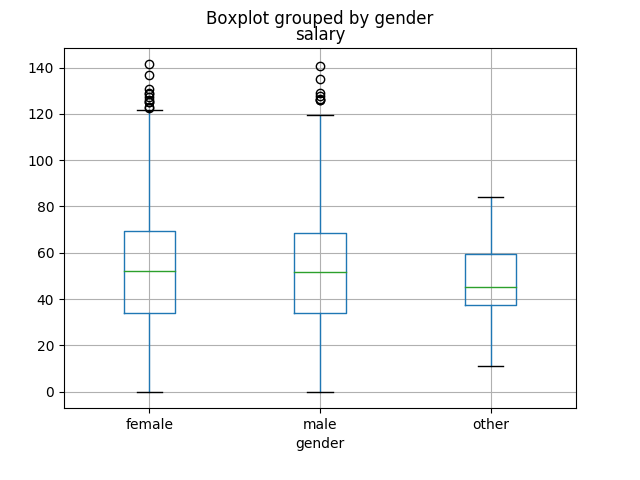
\includegraphics[width=0.45\textwidth]{genderSalary.png}
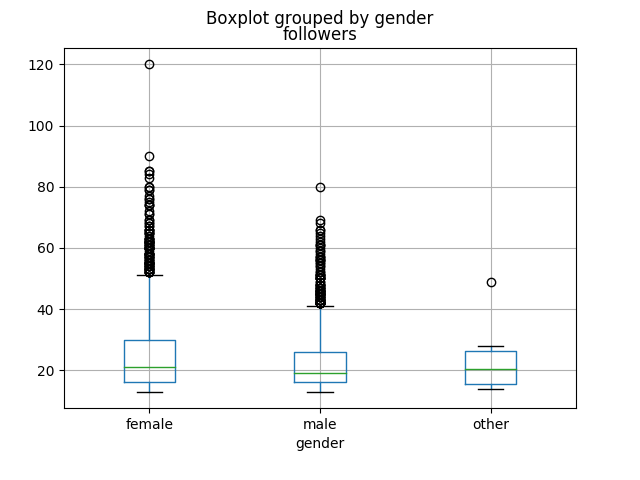
\includegraphics[width=0.45\textwidth]{genderFollowers.png}
\caption{Grouped box plots of salary (left) and number of social media
followers (right), grouped by gender.}
\label{fig:genderPlots}
\end{figure}

Similarly, we get the plot on the right-hand side with this code:

\begin{Verbatim}[fontsize=\small,samepage=true,frame=single,framesep=3mm]
people.boxplot('salary',by='followers')
\end{Verbatim}

This looks more skewed (\texttt{female}s appear to perhaps have more followers
on average than \texttt{male}s), but of course we won't know for sure until we
run the right statistical test.

\subsection{The $t$-test}

% TODO: F-test when there's more than two values for your categorical variable.

\index{t-test@\textit{t}-test}
\index{groupby@\texttt{.groupby()} method (Pandas)}
\index{bell-curvy@``bell-curvy''}

The test we'll use for significance here is called the \textbf{\textit{t}-test}
(sometimes ``Student's $t$-test'') and is used to determine whether the
\textit{means} of two groups are significantly different.\footnote{Strictly
speaking, the $t$-test assumes that the data sets you're comparing are ``bell
curvy'' (or ``normally distributed,'' to be precise) and we haven't checked for
that here. However, since we're doing \textit{exploratory} data analysis (not
drawing up and documenting final conclusions) it's common to use a $t$-test as
a quick-and-dirty just to see what's worth investigating.} Remember, we can get
the mean salary for each of the groups by using the \texttt{.groupby()} method:

\begin{Verbatim}[fontsize=\small,samepage=true,frame=single,framesep=3mm]
people.groupby('gender')['salary'].mean()
\end{Verbatim}
\vspace{-.2in}

\begin{Verbatim}[fontsize=\small,samepage=true,frame=leftline,framesep=5mm,framerule=1mm]
gender
female    52.031283
male      51.659983
other     48.757000
\end{Verbatim}

Females have the edge over males, 52.03 to 51.66. Our question is: is this
``enough'' of a difference to justify generalizing to the population?

To run the $t$-test, we first need a \texttt{Series} with just the
\texttt{male} salaries, and a different \texttt{Series} with just the
\texttt{female} salaries. These two \texttt{Series}es are \textit{not} usually
the same size. Let's use a query to get those:

\begin{Verbatim}[fontsize=\small,samepage=true,frame=single,framesep=3mm]
female_salaries = people[people.gender=="female"]['salary']
male_salaries = people[people.gender=="male"]['salary']
\end{Verbatim}
\vspace{-.2in}


\index{ttest\_ind@\texttt{ttest\_ind()} (SciPy)}

and then we can feed those as arguments to the \texttt{ttest\_ind()} function:

\begin{Verbatim}[fontsize=\small,samepage=true,frame=single,framesep=3mm]
scipy.stats.ttest_ind(female_salaries, male_salaries)
\end{Verbatim}
\vspace{-.2in}

\begin{Verbatim}[fontsize=\small,samepage=true,frame=leftline,framesep=5mm,framerule=1mm]
Ttest_indResult(statistic=0.5241138589648577, pvalue=0.6002226372421067)
\end{Verbatim}

This output is a bit more readable than the $\chi^2$ was. The second number in
that output is labeled ``\texttt{pvalue}'', which is over .05, and therefore we
conclude that \textit{there is no evidence that average salary differs between
males and females.}

Just to complete the thought, let's run this on the \texttt{followers} variable
instead:

\begin{Verbatim}[fontsize=\small,samepage=true,frame=single,framesep=3mm]
female_followers = people[people.gender=="female"]['followers']
male_followers = people[people.gender=="male"]['followers']
scipy.stats.ttest_ind(female_salaries, male_salaries)
\end{Verbatim}
\vspace{-.2in}

\begin{Verbatim}[fontsize=\small,samepage=true,frame=leftline,framesep=5mm,framerule=1mm]
Ttest_indResult(statistic=9.861473026659873, pvalue=9.857302431746571e-23)
\end{Verbatim}

\textbf{Warning!} When you first look at that $p$-value, you may be tempted to
say ``9.857 is \textit{waaay} greater than .05, so I guess this is a `no
evidence' result as well.'' Not so fast! If you look at the entire number --
including the ending -- you see:

\vspace{-.1in}
\begin{center}
\texttt{9.857302431746571e-23}
\end{center}
\vspace{-.1in}

\index{scientific notation}
\index{e@``\texttt{e}'' (exponential) notation}

that sneaky little ``\texttt{e-23}'' at the end is the kicker. This is how
Python displays numbers in \textbf{scientific notation} The
``\texttt{e}'' means ``times-ten-to-the.'' In mathematics, we'd write that
number as:

\vspace{-.2in}
\begin{center}
$9.857302431746571 \times 10^{-23}$
\end{center}
\vspace{-.2in}

which is:

\vspace{-.2in}
\begin{center}
$.000000000000000000000009857302431746571$
\end{center}
\vspace{-.2in}

Wow! That's clearly waaay \textit{less than} .05, and so we can say \textit{the
average number of followers \underline{does} depend significantly on the gender.}

Be careful with this. It's an easy mistake to make, and can lead to
embarrassingly wrong slides in presentations. \smiley


\section{Two numeric variables}

Finally, we have the case where both variables are numeric. The \texttt{salary}
and \texttt{followers} columns are this case. Are they associated?

\subsection{Scatter plots}
\index{scatter plot}

The correct plot to visualize this is the \textbf{scatter plot}. It has an
axis for each numeric variable, and plots one dot (or other marker) for each
object of study: its $x$/$y$ coordinates depend on that object's value for each
variable.

The Pandas code is as follows:

\begin{Verbatim}[fontsize=\small,samepage=true,frame=single,framesep=3mm]
people.plot.scatter(x='followers',y='salary')
\end{Verbatim}

which produces Figure~\ref{fig:followersSalary}. Interestingly, there appear to
be a lot of people pegged at zero salary, and also at 10-ish followers. (These
observations would have shown up in a univariate analysis as well.) There's no
super obvious connection between the two variables, but if you squint at the
plot it (maybe) looks like there's a slight up-and-to-the-right trend, which
would indicate that having more followers is modestly associated with earning
more money.

\begin{figure}[ht]
\centering
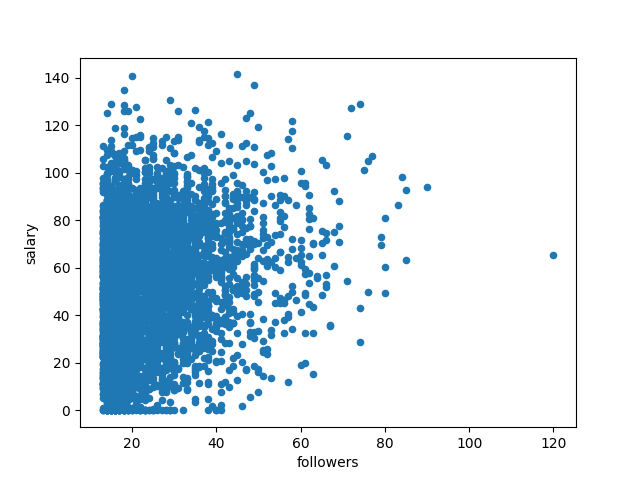
\includegraphics[width=0.8\textwidth]{followersSalary.png}
\caption{A scatter plot of \texttt{followers} vs.~\texttt{salary}. Each point
in the plot represents one person, with the $x$ and $y$ coordinates
corresponding to his/her/their number of followers and salary.}
\label{fig:followersSalary}
\end{figure}

\section{Pearson correlation coefficient}
\index{Pearson correlation coefficient}
\index{correlation coefficient}
\index{pearsonr@\texttt{pearsonr()} (SciPy)}

The test we'll use to see whether this pattern is significant is the
\textbf{Pearson correlation coefficient} (also called ``Pearson's $r$''). To
run it, we call SciPy's \texttt{pearsonr()} function and pass it the two
columns:

\begin{Verbatim}[fontsize=\small,samepage=true,frame=single,framesep=3mm]
scipy.stats.pearsonr(people.salary, people.followers)
\end{Verbatim}
\vspace{-.2in}

\begin{Verbatim}[fontsize=\small,samepage=true,frame=leftline,framesep=5mm,framerule=1mm]
(0.2007815176819964, 1.2285885030618397e-46)
\end{Verbatim}

We're given two numbers as output. The \textit{second} of these is the
$p$-value, and remembering our pitfall from above, we're savvy enough to notice
the \texttt{e-46} at the end and declare it significant. So we can say
\textit{we have high confidence that a person's salary is associated with their
number of social media followers.}

\index{positive correlation}
\index{negative correlation}

Now for the first number, which is the actual ``correlation coefficient.''
\textit{If} the second number is below $\alpha$ and therefore significant (as
it was here), you then look at the first number and see whether it's positive
or negative. Positive numbers indicate \textbf{positive correlations}: an
increase in one of the variables corresponds to an \textit{increase} in the
other. Negative numbers indicate \textbf{negative correlations}: an increase in
one of the variables corresponds to a \textit{decrease} in the other. Here, we
have a positive number, which means that \textit{having more followers tends to
go with a higher salary.}

As an example of the second (negative) case, suppose two of our variables in a
data set of sailboat races were \texttt{length} (the length of the sailboat,
from bow to stern) and \texttt{finish\_time} (the number of minutes the boat
took to complete the race). We're likely to see a negative correlation in this
case, because physics tells us that \textit{longer} boats can travel through
the water \textit{faster} (and therefore have \textit{lower} finish times).
These two variables would thus be correlated, but in a negative way: a high
value for one would typically indicate a \textit{low} value for the other.
